\documentclass[11pt,a4paper]{article}
\usepackage[T1]{fontenc}  
\usepackage[francais]{babel}
\usepackage[utf8]{inputenc}
\usepackage{pb-diagram} %                              pour construire des diagrammes commutatifs

%\usepackage{fancyhdr}
\pagestyle{plain}%                                             entête et pied de page
%\pagenumbering{arabic}%

%
\usepackage[vmargin=5cm]{geometry}%           marges en haut et en bas.

\setlength{\parskip}{5pt}%                                espace entre les paragraphes
%%x
%\setlength{\marginparwidth}{0.5cm}%
%\setlength{\hoffset}{-1in}%
%\setlength{\voffset}{-1in}%
%%\setlength{\evensidemargin}{1cm}%
%%\setlength{\oddsidemargin}{2cm}%
%\setlength{\textwidth}{17cm}%
%\setlength{\marginparsep}{0.1cm}%
%\setlength{\marginparwidth}{1.7cm}%
%\setlength{\topmargin}{1cm}%
%\setlength{\headheight}{1cm}%
%\setlength{\headsep}{1cm}%
%\setlength{\textheight}{24.0cm}%
%%
%\setlength{\oddsidemargin}{1.5cm}%
%\setlength{\evensidemargin}{1.5cm}%
%
\setlength{\parindent}{12pt}%                             indentation des paragraphes
%
\usepackage{color}%
\usepackage{mdwlist}%                                      pour liste
\usepackage{graphicx}%                                    insérer une image
%\usepackage{float}%                                           positionner des figures
\usepackage{here}
\usepackage{makeidx}%         				    pour faire index
\setcounter{secnumdepth}{3}%                      ??  numéroter les subsubsections
%
\usepackage{amsmath}%
\usepackage{amssymb}%
\usepackage{amsthm}%
\usepackage{amsfonts}%
\usepackage{mathrsfs}%
%\usepackage{bbm}%                                              lettres ensembles (N, Z, Q, R)
\usepackage[all,cmtip]{xy}%
%\xyoption{all}
\usepackage{rotate}%					       pivoter des objets
%\usepackage{yfonts}%                                            écritures gothiques, etc
%\usepackage{eurosans}
%\usepackage{mathabx}
%
\usepackage{graphicx}
\usepackage{caption}
\usepackage{eurosym}
%
\usepackage{array}% 
\usepackage{multirow}
%\usepackage[retainorgcmds]{IEEEtrantools}         					tableaux
%
\usepackage{natbib}
 
% fourier soit stmaryrd 
%\usepackage{fourier}
%Commandes d'environnement de théorèmes.
\newtheorem{Prop}{Proposition}[section]%
\newtheorem{Theo}[Prop]{Théorème}%                   la numérotation suit celle de 
\newtheorem{Def}[Prop]{Définition}%                      l'environnement "prop"
\newtheorem{Cor}[Prop]{Corollaire}%
\newtheorem{Lem}[Prop]{Lemme}%
\newtheorem{Conj}[Prop]{Conjecture}%
\newtheorem{Hyp}[Prop]{Hypothèse}%
\newtheorem{Question}[Prop]{Question}%
\newtheorem{Rq}[Prop]{Remarque}%
\newtheorem{Term}[Prop]{Terminologie}%
\newtheorem{Ex}[Prop]{Exemple}%
\newtheorem{Rap}[Prop]{Rappels}%
\newtheorem{PropDef}[Prop]{Proposition et définition}%
%
%[section]
%Lettres bb
\newcommand{\A}{\mathbb A}%
\newcommand{\C}{\mathbb C}%
\newcommand{\D}{\mathbb D}%
\newcommand{\E}{\mathbb E}%
\newcommand{\fp}{\mathbb F_{p}}%
\newcommand{\Fp}{\mathbb F}%
\newcommand{\G}{\mathbf G}%
\newcommand{\Gm}{\mathbb G}
\newcommand{\Hbb}{\mathbb H}
\newcommand{\N}{\mathbb N}%
\newcommand{\Pbb}{\mathbb P}%
\newcommand{\Q}{\mathbb Q}%
\newcommand{\qp}{\mathbb Q_{p}}%
\newcommand{\R}{\mathbb R}%
\newcommand{\Sun}{\mathbb S}%
\newcommand{\U}{\mathbb U}%
\newcommand{\Wm}{\mathbb W_{M}}%
\newcommand{\x}{\mathbf x}%
\newcommand{\W}{\mathbb W}%
\newcommand{\Z}{\mathbb Z}%
\newcommand{\zp}{\mathbb Z_{p}}%
\newcommand{\Zc}{\mathbf Z}%
%
%
%Lettres cal
\newcommand{\Acal}{\mathcal A}%
\newcommand{\Bcal}{\mathcal B}
\newcommand{\Ccal}{\mathcal C}%
\newcommand{\Dcal}{\mathcal D}%
\newcommand{\Ecal}{\mathcal{E}}%
\newcommand{\Fcal}{\mathcal F}%
\newcommand{\Gcal}{\mathcal G}%
\newcommand{\Hcal}{\mathcal H}%
\newcommand{\Ical}{\mathcal I}%
\newcommand{\Jcal}{\mathcal J}%
\newcommand{\Lcal}{\mathcal L}%
\newcommand{\Mcal}{\mathcal{M}}%
\newcommand{\Ncal}{\mathcal N}%
\newcommand{\Ocal}{\mathcal O}%
\newcommand{\Pcal}{\mathcal P}%
\newcommand{\Kcal}{\mathcal K}%
\newcommand{\Rcal}{\mathcal R}%
\newcommand{\Scal}{\mathcal S}%
\newcommand{\Tcal}{\mathcal T}%
\newcommand{\Ucal}{\mathcal U}%
\newcommand{\Vcal}{\mathcal V}%
\newcommand{\Wcal}{\mathcal W}%
\newcommand{\Xcal}{\mathcal X}%
\newcommand{\Xcalo}{\mathcal X_{0}}%
\newcommand{\Zcal}{\mathcal Z}%
%\newcommand{\Ochi}{\Orond_{\chi}}
%Lettre caligraphiée
\newcommand{\Acali}{\mathscr A}
\newcommand{\Bcali}{\mathscr B}%
\newcommand{\Ccali}{\mathscr C}%
\newcommand{\Dcali}{\mathscr D}%
\newcommand{\Fcali}{\mathscr F}%
\newcommand{\Icali}{\mathscr I}%
\newcommand{\Jcali}{\mathscr J}%
\newcommand{\Lcali}{\mathscr L}%
\newcommand{\Ncali}{\mathscr N}%
\newcommand{\Ocali}{\mathscr O}%
\newcommand{\Pcali}{\mathscr P}%
\newcommand{\Scali}{\mathscr S}%
\newcommand{\Tcali}{\mathscr T}%
\newcommand{\Vcali}{\mathscr V}%
\newcommand{\Xcali}{\mathscr X}%
\newcommand{\Ycali}{\mathscr Y}%
\newcommand{\Zcali}{\mathscr Z}%
%
%Lettres frak pour les idéaux
\newcommand{\aid}{\mathfrak a}%
\newcommand{\fid}{\mathfrak f}%
\newcommand{\rid}{\mathfrak r}%
\newcommand{\sid}{\mathfrak s}%
\newcommand{\tid}{\mathfrak t}%
\newcommand{\Nid}{\mathfrak N}%
\newcommand{\cid}{\mathfrak c}%
\newcommand{\qid}{\mathfrak q}%
\newcommand{\Qid}{\mathfrak Q}%
\newcommand{\pid}{\mathfrak p}%
\newcommand{\mgot}{\mathfrak m}%
\newcommand{\zid}{\mathfrak z}%
\newcommand{\Xfrak}{\mathfrak X}%%


%Expressions mathématiques communes
\newcommand{\somme}[2]{\underset{#1}{\overset{#2}\sum}}%
\newcommand{\produit}[2]{\underset{#1}{\overset{#2}\prod}}%
\newcommand{\produittenseur}[2]{\underset{#1}{\overset{#2}\bigotimes}}%
\newcommand{\union}[2]{\underset{#1}{\overset{#2}\bigcup}}%
\newcommand{\inter}[2]{\underset{#1}{\overset{#2}\bigcap}}%
\newcommand{\uniondisjointe}[2]{\underset{#1}{\overset{#2}\coprod}}%
\newcommand{\sommedirecte}[2]{\underset{#1}{\overset{#2}\bigoplus}}%
%

\newcommand{\binomial}[2]{\begin{pmatrix}#1\\#2\end{pmatrix}}

%test newcomand avec R double barre
\newcommand{\card}[1]{\overline{\overline{#1}}}
\newcommand{\cardR}{\card{\R}}
\newcommand{\cardBR}{\card{\Bcali(\R)}}
\newcommand{\deriv}{ \mathrm{d}}

\newcommand{\intervEntier}[1]{ $[\![$ {#1} $]\!]$ }

\graphicspath{{Pictures/}}


\newcommand{\FL}[1]{\textcolor{red}{#1}}
\newcommand{\GC}[1]{\textcolor{blue}{#1}}



%\bibliographystyle{elsarticle-harv} 

%Page de garde

 



%%%%%%%%%%%%%%%%%%%%%%%%%%%%%%%%%%%%%%%%%%%%%%%%%%%%%%%%%%%%%%%
%                                                                                                                                 %
%                                                        DEBUT                                                               %
%                                                                                                                                 %
%%%%%%%%%%%%%%%%%%%%%%%%%%%%%%%%%%%%%%%%%%%%%%%%%%%%%%%%%%%%%%%


\begin{document}

But du document: proposer un modèle pour l'étude de l'instrument développé par Laurent Bolognini: electra.

\section{Description de l'instrument}
Composé de 3 moteurs, de tiges et de lumières.
On peut agir sur la vitesse de rotation des 3 moteurs (et le sens) et l'intensité de chaque lumière.


\section{Objectifs}
\begin{itemize}
\item Caractériser les formes produites par l'instrument: on étudie plus la forme que l'intensité lumineuse ?
\item Trouver toutes celles qu'il est possible de créer.
\item Si on se donne une forme, est-on capable de la reproduire avec l'instrument, si oui, comment?
\end{itemize}

\section{Méthode}
Proposer un modèle de l'instrument. Un premier modèle consistera à décrire le mouvement dans son état non transitoire = stationnaire ? (donc sans variation des paramètres).
On pourra ensuite éventuellement prendre en compte la persistance rétinienne, et les régimes transitoires (donc la possibilité de faire varier la vitesse de moteurs).
L'implémenter et visualiser des réalisations du modèle.
Caractériser les sorties du modèle: trouver des mesures (pertinentes) qui diffèrent entre les résultats issus de paramètres différents.
Piste: utilisation du logiciel OpenMole (algorithme PSE) pour trouver les sorties atteignables: trouver le plus de configurations possibles qui donnent des résultats différents dans l'espace des mesures trouvées précédemment.


\section{Modèle}

\begin{figure}[H] 
\center{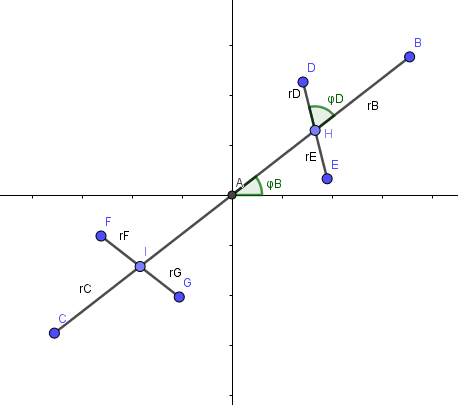
\includegraphics[width=0.75\linewidth]{schema2}}
\caption{Schéma du modèle}
\end{figure}


\subsection{Non transitoire}

\FL{Mettre un schéma, + une image de l'instrument?}

Paramètres fixes: 
rayons: $r_B$, $r_C$, $r_D$, $r_E$, $r_F$, $r_G$
 
"rayons" de points intermédiaires : $\alpha_H$, $\alpha_I$. 

Si $\alpha_H=1$, $H=B$, $\alpha_H=2$, $H$ est le milieu du segment $[BC]$, si $\alpha_H \rightarrow \infty$, $B=A$.


paramètres input: 
position initiale: angle: $\phi_B$, $\phi_D$, $\phi_F$
($+ \pi$ pour les points symétriques).

vitesse des moteurs: $v_1$, $v_2$, $v_3$ (nombre de tours par seconde) + sens de rotation

intensité lumineuse


On prend le point $A$ comme origine du repère.

Position des points en fonction du temps (et des positions initiales):

$A(x_A,y_A) = (0,0)$

$B(x_B,y_B) = (r_B \cos(2 \pi v_1 t + \phi_B),r_B \sin(2 \pi v_1 t + \phi_B))$

à $t=0$, $B = (r_B \cos(\phi_B), r_B \sin(\phi_B))$

$C(x_C,y_C) = (r_C \cos(2 \pi v_1 t + \phi_B + \pi),r_B \sin(2 \pi v_1 t + \phi_B + \pi))$

$H(x_H,y_H) = ( \frac{r_B}{\alpha_H} \cos(2 \pi v_1 t + \phi_B),\frac{r_B}{\alpha_H} \sin(2 \pi v_1 t + \phi_B))$

De même,
$I(x_I,y_I) = ( \frac{r_C}{\alpha_I} \cos(2 \pi v_1 t + \phi_B + \pi), \frac{r_C}{\alpha_I} \sin(2 \pi v_1 t + \phi_B + \pi))$

Pour déterminer la position des points $D,E,F,G$, on utilise les points intermédiaires ($H$ et $I$), (utilise le changement de repère  orthonormale centrée en H et de vecteurs directeurs un  de même direction que $\overrightarrow{AH}$, l'autre orthogonal, dans lequel $\overrightarrow{HD} =  rD( \cos(2 \pi v_2 t + \phi_D), \sin(2 \pi v_2 t + \phi_D))$ au repère usuel)

$ D(t) = (x_D(t),y_D(t)) = (\frac{r_B}{\alpha_H} \cos(2 \pi v_1 t + \phi_B) + r_D \cos(2 \pi (v_2 + v _1)t + (\phi_D + \phi_B)), \frac{r_B}{\alpha_H} \sin(2 \pi v_1 t + \phi_B ) + r_D \sin(2 \pi (v_2 +v_1)t +  (\phi_D + \phi_B))  )$

$
D=
\begin{pmatrix}
x(D) \\ 
y(D)
\end{pmatrix}
=
\begin{pmatrix}
\frac{r_B}{\alpha_H} \cos(2 \pi v_1 t + \phi_B) + r_D \cos(2 \pi (v_2 + v _1)t + (\phi_D + \phi_B) \\ 
\frac{r_B}{\alpha_H} \sin(2 \pi v_1 t + \phi_B ) + r_D \sin(2 \pi (v_2 +v_1)t +  (\phi_D + \phi_B))  
\end{pmatrix}
$

%$ \overrightarrow{HD} = (r_D \cos(2 \pi v_2 t + \phi_D),r_D \sin(2 \pi v_2 t + \phi_D))$
%
%
%Donc  $ \overrightarrow{AD} = \overrightarrow{AH} + \overrightarrow{HD} = (\frac{r_B}{\alpha_H} \cos(2 \pi v_1 t + \phi_B) + r_D \cos(2 \pi v_2 t + \phi_D), \frac{r_B}{\alpha_H} \sin(2 \pi v_1 t + \phi_B)) + r_D \sin(2 \pi v_2 t + \phi_D)  )$
%
%Donc $ D = (x_D,y_D) = (\frac{r_B}{\alpha_H} \cos(2 \pi v_1 t + \phi_B) + r_D \cos(2 \pi v_2 t + \phi_D), \frac{r_B}{\alpha_H} \sin(2 \pi v_1 t + \phi_B)) + r_D \sin(2 \pi v_2 t + \phi_D)  )$


Vitesse de $D$ au temps $t$:

$ D'(t) = (x'_D(t),y'_D(t)) = (-\frac{r_B}{\alpha_H} 2 \pi v_1 \sin(2 \pi v_1 t + \phi_B) - r_D 2 \pi (v_2 + v _1) \sin(2 \pi (v_2 + v _1)t + (\phi_D + \phi_B)), \frac{r_B}{\alpha_H} 2 \pi  v_1 \cos(2 \pi v_1 t + \phi_B ) + r_D  2 \pi (v_2 + v _1) \cos(2 \pi (v_2 +v_1)t +  (\phi_D + \phi_B))  )$



Accélération de $D$ au temps $t$:

$ D''(t) = (x''_D(t),y''_D(t)) = (-\frac{r_B}{\alpha_H} (2 \pi v_1)^2 \cos(2 \pi v_1 t + \phi_B) - r_D  (2 \pi (v_2 + v _1))^2 \cos(2 \pi (v_2 + v _1)t + (\phi_D + \phi_B)), - \frac{r_B}{\alpha_H} (2 \pi  v_1)^2 \sin(2 \pi v_1 t + \phi_B ) - r_D  (2 \pi (v_2 + v _1))^2 \sin(2 \pi (v_2 +v_1)t +  (\phi_D + \phi_B))  )$



Remarque: soit $\alpha \in \R$, (pour tout $v_1,v_2,t$)

$B(\alpha v_1,t) = B(v_1,\alpha t)$,

$D(\alpha v_1,\alpha v_2,t) = D(v_1,v_2,\alpha t)$

Donc multiplier les 3 vitesses par un facteur identique ne changera pas la figure totale obtenue (l'image de tout les temps): il existe un temps (et on sait lequel), auquel le point sera au même endroit que pour l'autre vitesse. Une différence peut intervenir si l'on considère la persistance rétinienne.




\subsection{Persistance rétinienne}

Il semblerait que l’oeil garde une image rémanente pendant 1/25 seconde sur la rétine.

Dans le modèle, cela reviendrait non pas à avoir en sortie à l'instant $t$ la position des lumières à cet instant, mais l'ensemble des positions des lumières occupées durant les 1/25 secondes précédentes. Remarque, plus les vitesses des moteurs (donc de déplacement des lumières) sont importantes, plus les lumières parcourent de distance pendant ces 1/25 secondes, et donc plus les figurent ont une grande "longueur".


\subsection{Non transitoire}

piste ? Relier la tension d'entrée du moteur à la sortie: vitesse angulaire. L'idée serait que quand on tourne le bouton, on fait varier la tension du moteur et donc sa vitesse (prendre en compte l'inertie). On pourrait donc chercher des fonction du temps comme contrôle du système (la position du bouton de contrôle du moteur).


\section{Étude mathématique}
Courbe paramétrée pour la dynamique de chacun de points. On se concentre d'abord sur la courbe paramétrée produite par un point, on pourra ensuite éventuellement s'intéresser à la figure produite par tous les points (union des courbes paramétrées).

Étude des points singulier: condition nécessaire pour en avoir.

Étude de la périodicité: condition suffisante si il existe $m,n \in \N$ tels que $ \frac{m}{v_1}= \frac{n}{v_2}$. 

Étude de de la monotonie de chaque composantes ($x$ et $y$) 

Points doubles: $t_1$ et $t_2$ tels que: $x(t_1)=x(t_2)$ et $y(t_1) = y(t_2)$.



\section{Mesures}
La corube est elle fermée (périodicité)

boucles

point de rebroussement

ligne droite


%%%%%%%%%%%%%%%%%%           END      %%%%%%%%%%%%%%%%%%%%%%%%%%%%%%%%%

 
\end{document}

